%% uctest.tex 11/3/94
%% Copyright (C) 1988-2004 Daniel Gildea, BBF, Ethan Munson.
%
% This work may be distributed and/or modified under the
% conditions of the LaTeX Project Public License, either version 1.3
% of this license or (at your option) any later version.
% The latest version of this license is in
%   http://www.latex-project.org/lppl.txt
% and version 1.3 or later is part of all distributions of LaTeX
% version 2003/12/01 or later.
%
% This work has the LPPL maintenance status "maintained".
% 
% The Current Maintainer of this work is Daniel Gildea.

\documentclass[11pt]{ucthesis}
\def\dsp{\def\baselinestretch{1.5}\large\normalsize}
\dsp
\usepackage{graphicx}
% \usepackage{hyperref}
\usepackage[hidelinks]{hyperref}
\begin{document}

% Declarations for Front Matter

\title{Using haplotype information to sample and index pangenomes}
\author{Parsa Eskandar}
\degreeyear{2024}
\degreemonth{August}
\degree{DOCTOR OF PHILOSOPHY}
\chair{Professor Russ Corbett-Detig}
\committeememberone{Professor Benedict Paten}
\committeemembertwo{Professor Karen Miga}
\committeememberthree{Professor Heiner Litz}
\committeememberfour{Doctor Jouni L Siren}
\numberofmembers{5} %% (including chair) possible: 3, 4, 5, 6
\deanlineone{Peter Biehl}
\deanlinetwo{Vice Provost and Dean of Graduate Studies}
% \deanlinethree{}
\field{Biomolecular Engineering And Bioinformatics}
\campus{Santa Cruz}

\begin{frontmatter}

\maketitle
\copyrightpage

\tableofcontents
\listoffigures
% \listoftables

\begin{abstract}
The human reference genome has been a cornerstone of biological research, yet its limited diversity restricts its applicability across different populations. Pangenomes, which incorporate genetic variations from diverse individuals, offer a more inclusive alternative, but their complexity poses significant computational challenges. In my research, I will develop innovative computational tools to address these challenges. First, I will create a haplotype sampling technique to generate personalized pangenome references, enhancing accuracy in mapping and variant calling. Next, I will design a novel graph indexing structure to efficiently store and retrieve data from pangenomes, reducing computational overhead. Finally, I will improve Moni-align, an advanced pangenome aligner. Integrating these advancements can optimize its performance for large-scale genomic analyses. These contributions aim to make pangenome-based analyses more reliable and accessible, advancing the field of genomics.

\end{abstract}

% \begin{dedication}
% \null\vfil
% {\large
% \begin{center}
% To myself,\\\vspace{12pt}
% Perry H. Disdainful,\\\vspace{12pt}
% the only person worthy of my company.
% \end{center}}
% \vfil\null
% \end{dedication}


\begin{acknowledgements}
I want to thank my advisor, Benedict Paten, for his guidance and support throughout my PhD. A special thanks to my mentor, Jouni Sirén, for his valuable insights and constant help. I'm also grateful to my labmates in the CGL for their collaboration and excellent feedback. Finally, I appreciate Russ Corbett-Detig, Karen Miga, and Heiner Litz for serving on my committee.
\end{acknowledgements}

\end{frontmatter}

% \part{First Part}

\chapter*{Introduction}

The traditional linear reference genome, which represents a single consensus sequence as a standard for a species, has been instrumental in advancing genomic research. However, this linearity inherently introduces biases that limit its effectiveness. The human reference genome is a linear genome representing a single haplotype copy of the genome. Therefore, it does not adequately capture the full spectrum of human genetic diversity. As a result, using this reference can lead to incomplete or inaccurate representations of the genomes of individuals from other populations. This bias affects various applications, from genetic association studies to identifying structural variations, leading to potential misinterpretations and missed discoveries.\\
A pangenome addresses the limitations of the linear reference by encompassing the set of genomic variations present within a species. Rather than relying on a single, linear sequence, a pangenome includes multiple reference sequences representing the diversity of genomes across different individuals and populations. This comprehensive approach allows researchers to study the entire spectrum of genetic variations, including rare or population-specific ones. Therefore, the biases introduced by a single linear reference are reduced. By integrating more diverse sequences, a pangenome offers a more accurate and inclusive representation of a species' genetic landscape, enabling better insights into genetic diversity, evolution, and disease susceptibility.\\
Building on the concept of a pangenome, a pangenome graph represents this comprehensive set of sequences in a graph-based structure, where nodes represent genomic sequences and edges represent the relationships between them. This structure is compelling because it allows for the visualization and analysis of complex variations, such as insertions, deletions, and rearrangements, which are often oversimplified or missed entirely when using a linear reference. The pangenome graph can capture a species' full range of genetic diversity, providing a more nuanced and accurate model for genomic analyses. By enabling the alignment of individual genomes against this graph, researchers can more precisely identify genetic variations, leading to improved accuracy in genomic studies and a deeper understanding of genetic contributions to health and disease. One popular way of representing pangenomes is using variation graphs (vg) \cite{garrison2018variation}. Variation graphs are sequence graphs that additionally encode a set of reference paths through the graph. Each node in the graph is labeled with a sequence, and each path represents a sequence by concatenating the node sequences.\\
The Human Pangenome Reference Consortium (HPRC) recently published a pangenome consisting of nearly complete genomes from 47 people from diverse origins \cite{liao2023draft,wang2022human}. Their plan is to include 350 genomes in their next release. However, even with 350 full genomes in the pangenome, it still contains a small subset of human genetic diversity. So, there will be pressure for a pangenome consisting of at least thousands of genomes.\\
Pangenomes reduce the biases compared to the linear references, but the variants in the pangenome that are not part of the sample can be misleading. These extra variants can cause false read mappings and reduce the accuracy of the mapper. These irrelevant variants are generally rarer in terms of allele frequency. The frequency filtering on the pangenomes is a way that was previously used to deal with these variants \cite{liao2023draft}. However, this is a blunt heuristic that both fails to remove some irrelevant variants and removes many relevant variants.\\
One of the main challenges in leveraging pangenomes lies in constructing and indexing these complex graphs. Unlike linear genomes, pangenome graphs must account for a multitude of variations and structural complexities. The first aim is to address this challenge by developing haplotype sampling techniques that create personalized pangenome references. By sampling relevant haplotypes based on k-mer counts in sequencing reads, this approach aims to enhance the representation of genetic diversity and improve the precision of genomic analyses.\\
The methodology proposed for haplotype sampling focuses on selecting haplotypes that closely match the sequenced genome, thus creating a subgraph that is a more accurate representation of the individual's genetic makeup. This personalized approach is tailored for use with vg graph-based aligner, Giraffe \cite{siren2021pangenomics}. Results indicate that this method not only improves mapping accuracy but also enhances variant calling and genotyping performance.\\
The second aim addresses the need for efficient indexing of pangenomes. Effective indexing is crucial for the rapid retrieval and analysis of genomic data, especially as the scale of pangenome projects continues to expand. Traditional indexing methods designed for linear genomes are inadequate for pangenomes due to the pangenome's complexity and the vast amount of data they encompass. With this aim, I propose the development of a novel graph indexer that leverages haplotype information to enable efficient storage, retrieval, and mapping of genomic data.\\
In Aim 3, I focus on enhancing the performance and accuracy of Moni-align \cite{rossi2022moni}, a cutting-edge pangenome aligner. Moni-aligner is the first full-fledged short-read pangenome aligner built on the r-index. Moni-align, while effective, struggles with memory inefficiency and slower speeds. Our approach leverages pangenome graphs' structural advantages, reducing memory usage without sacrificing alignment accuracy. By focusing on maintaining informative reads through efficient filtering, this aim seeks to advance Moni-align's capabilities, enabling it to handle larger pangenomes and improve the precision of human genomic analyses.\\
For the first two aims, I will contribute to vg, a toolkit for working with the variation graph representation of the pangenomes. I will contribute to Moni-align by improving it's filtering method for the third aim. 

\chapter{Aim1: Haplotype Sampling Pangenome}

\section{Introduction}


\\
In this Aim we introduce a new filtering approach, that imputes a personalized pangenome subgraph based on sampling local haplotypes according to k-mer counts in the reads. By selecting relevant haplotypes based on the sequence data, haplotype sampling enhances the representation of genetic diversity and improves the precision of genomic analyses. \\
My first aim is to create haplotype sampling techniques and demonstrate their application in creating personalized pangenome references. This involves developing methods to accurately sample relevant haplotypes based on k-mer counts, evaluating the performance of these methods, and comparing them to existing approaches. \\
My primary contribution was conducting a comprehensive evaluation of small variant calling using haplotype sampling. I executed and compared different pipelines. I ran the GATK best-practice pipeline and BWA-MEM paired with DeepVariant as the variant caller to benchmark the performance of the haplotype sampling. Also, to facilitate and streamline these haplotype sampling processes, I created workflows. These workflows make running haplotype sampling easier without having to get deep into the details. 
\section{Background}
Pangenome graphs \cite{eizenga2020pangenome} represent aligned haplotype sequences. Each node in the graph is labeled with a sequence, and each path represents the sequence obtained by concatenating the node labels.
While any path in the graph is a potential haplotype, most paths are unlikely recombination of true haplotypes. \\ 
One common application for pangenome graphs is to use them as a reference for read mapping \cite{rautiainen2020graphaligner,siren2021pangenomics,garrison2018variation}. Graph-based aligners tend to be more accurate than aligners using a linear reference sequence when
mapping reads to regions where the sequenced genome differs from the reference sequence. If the graph contains another haplotype close enough to the sequenced genome in that region, the aligner
can usually find the correct mapping. On the other hand, sequence variation that is present in the graph but not in the sequenced genome can make the aligner less accurate. Such variation can
imitate other regions, making incorrect mappings more likely.
Because having the right variants in the graph has a greater effect on mapping accuracy than having variants not present in the sequenced genome, the usual approach is building a graph based
on common variants only. The vg short read aligner got best results with the 1000 Genomes Project (1000GP) \cite{10002015global} graph when variants below 1\% threshold were left out.\\
The Giraffe short read aligner \cite{siren2021pangenomics} uses another approach for avoiding rare variants. As a haplotype-aware aligner, Giraffe can generate synthetic haplotypes by sampling local haplotypes proportionally with a greedy algorithm. It got best results with the 1000GP graph by generating 64 haplotypes. However, frequency filtering was still used with the Human Pangenome Reference Consortium (HPRC) subgraph intended for Giraffe. As the initial graphs contain only 90
haplotypes, the threshold was set to 10\%.\\
In my first aim, we propose a more direct approach with less overhead by creating a personalized pangenome reference through haplotype sampling. This method involves selecting haplotypes that are similar to the sequenced genome based on k-mer counts in the reads. By working directly with assembled haplotypes and maintaining phasing within 10 kbp blocks, the resulting sampled graph is a subgraph of the original graph, ensuring that any alignments in the sampled graph are also valid in the original graph.
This approach is tailored for the Giraffe aligner, which can quickly build the necessary indexes for read mapping. The method assumes a graph with a linear high-level structure, such as those built using the Minigraph–Cactus \cite{hickey2024pangenome} pipeline, and requires a high read coverage (at least 20x) to reliably classify k-mers into absent, heterozygous, and homozygous categories.
\\
When applied to HPRC graphs, this sampling approach increases the overall pipeline running time by less than 15 minutes. The sampled graph proves to be a better mapping target than the universal frequency-filtered graph, resulting in a small improvement in the accuracy of calling small variants with DeepVariant \cite{poplin2018universal} and a significant increase in the accuracy of genotyping structural variants (SVs) with vg \cite{hickey2020genotyping} and PanGenie \cite{ebler2022pangenome}. This method offers a more accurate and efficient framework for genomic analyses, reducing reference bias and enhancing the precision of variant calling and genotyping.

\section{Methods}

\subsection{Bidirected Pangenome Graphs}
Human pangenome graphs are typically constructed using the bidirected sequence graph model. In this model, nodes have unique identifiers and contain sequences. Edges, which are undirected, connect the sides of two nodes. A forward traversal of a node involves entering from the left side, reading the sequence, and exiting from the right side. Conversely, a reverse traversal enters from the right side, reads the reverse complement of the sequence, and exits from the left side.
There are multiple file formats for storing these bidirectional sequenced graphs. One of which is the text based Graphical Fragment Assembly (GFA) format. The GFA format is designed to represent sequence graphs as the outcome of an assembly, depicting genomic variations, splice graphs in genes, or overlaps between reads from long-read sequencing technology. A space-efficient binary format for pangenome graphs is the GBZ file format \cite{siren2022gbz}, which is based on the GBWT index \cite{siren2020haplotype}. The GBWT index stores haplotype paths as sequences of nodes. GBZ files are compatible with a subset of GFA, allowing for efficient conversion between the two formats.
The hierarchical structure of a bidirected sequence graph can be described using its snarl decomposition \cite{paten2018superbubbles}. A snarl, which is a generalization of a bubble \cite{zerbino2008velvet}, represents a site of genomic variation and is a subgraph that is separated by two node sides from the rest of the graph. Each snarl must be minimal, meaning neither of the sides defining it forms a snarl with a node side located within the subgraph. The entire graph can be decomposed into a series of chains, each consisting of nodes and snarls. A snarl may be primitive, or it may be further decomposed into additional chains.


\subsection{Preprocessing haplotypes}
We begin with the graph in the GBZ format. While this format is efficient in terms of space and query performance, it is not optimal for selecting haplotypes based on sequence similarity. Therefore, it is necessary to preprocess the graph and store the haplotypes in a more appropriate format.
Our preprocessing approach follows a method similar to that used in PanGenie (Figure \ref{fig:1:1}(A)). We treat each weakly connected component in the graph as a single top-level chain in the snarl decomposition. Unlike PanGenie, which combines bubbles less than 31 base pairs apart, we merge adjacent snarls in the top-level chains into blocks of roughly 10,000 base pairs. A minimum distance index \cite{chang2020distance} helps determine the length of these blocks.
Top-level chains usually correspond to chromosomes or other significant contigs. By dividing each top-level chain into a sequence of blocks, we ensure that sampled haplotype paths visit the same blocks in a consistent order. When haplotypes are sampled independently within each block, any recombination of these haplotypes is considered plausible. Although the graph has a linear high-level structure, it can contain reversals that allow the same haplotype to visit the same blocks multiple times. To prevent unbalanced recombinations, we consider each minimal end-to-end traversal of a block as a distinct haplotype. We efficiently identify these traversals by listing the paths that visit the border nodes of a block using the r-index \cite{gagie2020fully} and matching the node visits at both ends.
We describe the haplotypes in each block using block-specific k-mers (Figure \ref{fig:1:1}(B)). Unlike PanGenie, which uses k-mers with at most one hit per haplotype, we use minimizers with a single hit in the graph. We exclude uninformative k-mers that appear in all haplotypes. For each block, we create a k-mer presence matrix, a binary matrix indicating whether each selected graph-unique k-mer is present or absent in each haplotype.

\subsection{Sampling Haplotypes}
\subsubsection{K-mer classification}
The first step of haplotype sampling is to count k-mers in the reads and classify them (Figure \ref{fig:1:1}(C)). In the current workflow, we are using the KMC tool \cite{kokot2017kmc}, which counts k-mers from FASTQ/FASTA files. It is possible to use any other k-mer counting tool that uses the K-mer File Format (KFF) \cite{dufresne2022k}. In this algorithm we combine the counts of a k-mer with its reverse complement. We also ignore the k-mers that occurred only once in the reads as they might happen because of an error in the sequencing. Given the k-mer coverage and k-mer counts, we classify each k-mer as absent, heterozygous, homozygous, or frequent. We then ignore the frequent ones, because they are not informative for distinguishing between different haplotypes. If the k-mer coverage is not provided, we estimate it from the counts. For estimating the k-mer coverage, we use the distribution of the counts of the  present k-mers. Then we calculate the most common count among the k-mers. If the most common k-mer count is greater than the median count, we assume that most k-mers that are present in the sample are homozygous and will use this most common k-mer count as the coverage. Otherwise, if there is a secondary peak above the median at about 2x the primary peak, we use that. 
\subsubsection{Sampling process}
We sample the haplotypes independently in each block (Figure \ref{fig:1:1}(D)). We use a greedy algorithm to sample the haplotypes. We score the haplotypes by summing the scores of the k-mers. Each homozygous k-mer score is +1 or -1, depending on if it is present or absent in the haplotype. Each absent k-mer score is 0.8 or -0.8 respectively. Heterozygous haplotypes do not contribute to the scores. 
The haplotype sampling process starts with selecting an approximation of the consensus sequence as the first haplotype. For the following haplotypes, the goal is to cover all the homozygous k-mers while also choosing haplotypes that include or exclude heterozygous k-mers. We changed the score of the homozygous k-mers that were present in the selected haplotype by a multiplicative factor 0.9. This reduction means that these k-mers are less likely to influence the selection of future haplotypes because they are already covered.We also adjust the scores of the heterozygous k-mers by an additive term 0.05, making it more likely that the next haplotype is the opposite with respect to the presence of this k-mer. \\
We can either use the selected n haplotypes (n between 4 and 32), or use them as candidates for diploid sampling. For diploid sampling, we consider each pair of candidates and select the highest-scoring pair. For each k-mer, we find the number of copies we expect based on the k-mer counts x (0, 1, or 2) and the actual number of copies y. Then we define the score of that k-mer as $1 - |x-y|$ and the score for the pair is the sum of k-mer scores.\\
The next step after sampling local haplotypes near top level chains, is to combine them to form a full-length haplotype. We connect those adjacent blocks that the sampled haplotypes are the same. In other cases that they are not from the same haplotypes, the haplotypes we form are arbitrary recombinations of the local haplotypes we sampled.
If we want to include the reference path in the personalized pangenome, we insert the haplotypes into an empty GBWT index, along with the reference path. Otherwise we just add them to an empty GBWT index. 

\begin{figure}[H]
    \centering
    \includegraphics[width=\linewidth]{Images/figure1.pdf}
    \caption[Illustrating haplotype sampling at adjacent blocks in the pangenome]{\textbf{Illustrating haplotype sampling at adjacent blocks in the pangenome.} (A) A variation
graph representing adjacent locations in the pangenome, composed of a bidirected sequence graph (top) and
a set of embedded haplotypes (below); the dotted lines represent the boundary between the two blocks.
(B) k-mers that occur once within the graph, termed graph-unique k-mers, are identified in the haplotypes;
here k = 5 and graph-unique k-mers are colored red. (C) The graph-unique k-mers are counted in the reads, and based upon
counts classified as present, likely heterozygous (shown in orange), present, likely homozygous (shown in
blue), or absent (all red kmers in (B) not identified in the reads). (D) Using the identified graph-unique
k-mer classifications, a subset of haplotypes are selected at each location, defining a personalized pangenome
reference subgraph of the larger graph. Where needed, recombinations are introduced (see lightning bolt) to
create contiguous haplotypes.}
    \label{fig:1:1}
\end{figure}

\section{Results}
\subsection{Mapping reads}
We have done these benchmarkings in an AWS i4i.16xlarge with 32 cpus and 512 GiBs memory. We aligned 30x NovaSeq reads \cite{baid2020extensive} for the Genome in a Bottle (GIAB) \cite{wagner2022benchmarking} HG002 sample to various references using Giraffe and measured the running time. We used BWA-MEM \cite{li2013aligning} with GRCh38 reference as the baseline. The haplotype sampling first creates a sampled graph for HG002. Then we used KMC for counting the k-mers in the reads. We tested the haplotype sampling with 4, 8, 12, and 32 haplotypes as well as diploid sampling using 32 candidates. Giraffe also require distance index and and minimizer index, so whenever using a haplotype sampled graph, they needed to be built which added to the runtime of the pipeline. Figure \ref{fig:1:2} shows that Giraffe which uses graphs as reference is faster than BWA-MEM that uses linear reference. Furthermore, giraffe is more likely to find an exact (i.e. all-matches) alignment with the v1.1 diploid graph than with the frequency-filtered graphs, and the reads are more likely to be properly paired. It is also more confident about the alignments to the v1.1 diploid graph, as evidenced by the higher proportion of reads with mapping quality (Mapq) 60. The variant calling and genotyping results in the following sections show this confidence is well-founded.

\begin{figure}[h]
    \centering
    \includegraphics[width=\linewidth]{Images/figure2.pdf}
    \caption[Mapping 30x NovaSeq reads for HG002 to GRCh38 (with BWA-MEM) and to HPRC graphs (with Giraffe)]{\textbf{Mapping 30x NovaSeq reads for HG002 to GRCh38 (with BWA-MEM) and to HPRC graphs (with Giraffe).} The graphs (y-axis) are Minigraph–Cactus graphs built using GRCh38 as the
reference. For the sampled graphs, we tested sampling 4, 8, 16, and 32 haplotypes. For the v1.1 diploid
graph, 32 candidate haplotypes were used for diploid sampling. We show the overall running time and the
time spent for mapping only (left), and the fraction of reads with an exact, gapless, properly paired, and
mapping quality 60 alignment.}
    \label{fig:1:2}
\end{figure}


\subsection{Calling Small Variants}

I also evaluated the impact of haplotype sampling on the accuracy of calling small variants. I used the GIAB v4.2.1 GRCh38 benchmark set. I mapped PCR-free NovaSeq 40x \cite{wagner2022benchmarking} reads with Giraffe and called variants using DeepVariant \cite{poplin2018universal}, using the pipeline discussed in Liao et al. \cite{liao2023draft} Then I evaluated the results of the mapping using hap.py. Figure \ref{fig:1:3}(A) shows that the v1.1 diploid graph consistently outperformed the other graph configurations, reducing total errors by 9.1\% across samples HG001 to HG005 relative to the v1.1 filtered graph. I also compared the performance to mapping to a linear reference (GRCh38) with BWA-MEM \cite{li2013aligning} and using DeepVariant to call variants, as well as to the GATK best-practice pipeline \cite{poplin2017scaling}. (\ref{fig:1:3}(B))
Mapping the same NovaSeq 40x data to the v1.1 diploid graph with Giraffe reduced errors by an average 35\% relative to BWA-MEM/GRCh38, and 74\% (a near four-fold reduction in total errors) relative to the GATK best-practice.
\begin{figure}[h]
    \centering
    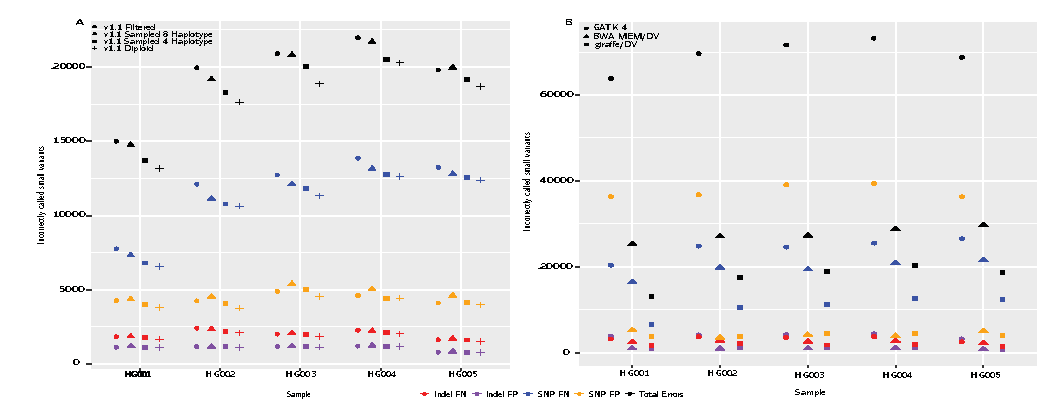
\includegraphics[width=\linewidth]{Images/figure3-1.pdf}
    \caption[Small Variants evaluation across samples HG001 to HG005]{\textbf{Small Variants evaluation across samples HG001 to HG005.} (A) The number of false
positive (FPs) and false negative (FNs) indels and SNPs across four different graphs, each using GRCh38
as the reference: v1.1 filtered, v1.1 sampled with 4 and 8 haplotypes, and v1.1 diploid, using the Giraffe/
DeepVariant pipeline. (B) Comparing the Giraffe/DeepVariant using the v1.1 diploid graph to BWA
MEM/DeepVariant and GATK best practice pipelines, both using the GRCh38 reference.}
    \label{fig:1:3}
\end{figure}

I further assessed the specificity of variant calling by comparing the incidence of false variants among three different tools across variants that are both present in the pangenome and in the NIST benchmark, as well as those exclusively in the NIST benchmark but absent from the pangenome (Figure \ref{fig:1:4}).
This analysis was crucial for understanding the performance of the tools on genomic variants that do not directly correspond to those represented within the pangenome graph. For the variants not included in the pangenome, v1.1 diploid shows 82\% improvement relative to GATK best-practice and 26\% improvement relative to BWA-MEM/GRCh38.

\begin{figure}[h]
    \centering
    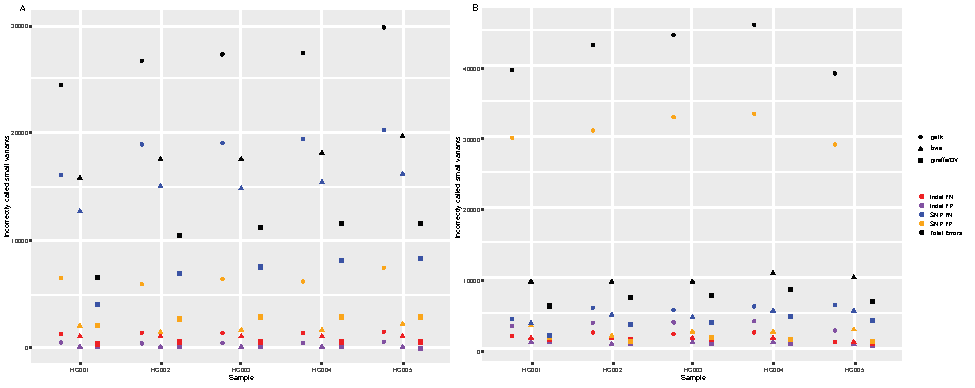
\includegraphics[width=\linewidth]{Images/in_out_pangenome (3).pdf}
        \caption[Small variant evaluation for variants included/not included in the pangenome]{\textbf{Small variant evaluation for variants included/not included in the pangenome.} (A) comparing the number of falsely called variants among the variants that occurred in the pangenome for different tools GATK, BWA MEM, vg giraffe (B) Comparing the falsely called variants among the variants that did not occur in the pangenome.}
    \label{fig:1:4}
\end{figure}


\subsection{Genotyping structural variants}
We evaluated the effectiveness of pangenome structural variant (SV) genotyping algorithms (using both PanGenie \cite{ebler2022pangenome} and vg call \cite{hickey2020genotyping}), for various pangenome graphs. Our assessment employed the GIAB Tier1 v0.6 truth set, which includes the confident structural variants for the HG002 sample. Haplotype sampling demonstrated an improvement in genotyping performance compared to both the v1.1 default and v1.1 filtered graphs (Figure \ref{fig:1:5}). Notably, the combination of v1.1 graphs and haplotype sampling significantly outperformed the v1.0 graphs described by Liao et al. Using PanGenie, the F1 score for variant calls increased from 0.7780 with the v1.0 filtered graph to 0.8926 with the v1.1 diploid graph. Also, using haplotype sampling with v1.1 diploid graph shows 0.375 improvement on F1 score that shows the effectiveness of haplotype sampling.  

\begin{figure}[h]
    \centering
    \includegraphics[width=\linewidth]{Images/figure4.pdf}
    \caption[SVs benchmark evaluation]{\textbf{SVs benchmark evaluation.} (A) Precision, recall, and F1 scores of both vg call and PanGenie
for different pangenome reference graphs on the GIAB v0.6 Tier1 call set. Graphs were built using GRCh38
as the reference.}
    \label{fig:1:5}
\end{figure}

\section{Conclusion}
We have developed a k-mer-based method for sampling local haplotypes that are similar to a sequenced genome. The results show that the haplotype sampled graphs are superior to the unfiltered and the frequency filtered graphs in different aspects. The graph resulted from this approach,  improved small variant calling and structural variant genotyping in comparison to the other graphs. Looking forward, we expect pangenomes from the HPRC and elsewhere to substantially grow in genome number, perhaps into the thousands of haplotypes over the next several years. Methods for personalizing pangenomes will therefore increase in importance as the fraction of all variation that is rare within them naturally expands. So, we expect the relevance and power of the personalization methods of the type introduced here to become increasingly vital to pangenome workflows.














\chapter{Aim2: Pangenome graph indexing}

\section{Introduction}

Indexing is essential in many bioinformatics applications, as it can greatly reduces the computational time and resources required for sequence alignment. Indexing allows the alignment algorithm to quickly locate the query sequences in the reference genome without having to search the entire genome for matches. Therefore, Effective indexing methods are essential for leveraging the full potential of pangenome graphs in genomic research. \\
In the current state of the HPRC pangenome, which contains 47 human genomes, we can still use the standard read aligners such as BWA-MEM \cite{li2013aligning} and Bowtie \cite{langmead2009ultrafast}. We might still be able to use these read aligners with 350 genomes using high-end supercomputers in next release. However, in the next steps, indexing thousands of genomes requires new data structures and new methods. To handle this amount of data, researchers use pangenome graphs, which show the variations between genomes as detours on an otherwise shared path. The necessity of mapping reads to the pangenome graph, which includes finding the best fitting position, leads to the question of how to index pangenome graphs.\\ 
Recently, Bal´az et al. \cite{balavz2024wheeler} introduced a new theoretical method called Wheeler maps. A Wheeler map stores a text T[1..n] and an assignment of tags to the characters of T called tag arrays such that we can preprocess a pattern P[1..m] and then, given i and j, quickly return all the distinct tags labeling the first characters of the occurrences of P[i..j] in T. This method can preprocess a pattern P[1..m] in O(mlogn) and then return the k distinct tags for the pattern in optimal O(k) time for any given i, and j. \\
This paper shows the theoretical basis for the Wheeler map. However, the full implementation of the data structures described in this paper, building efficient algorithms for extracting tag arrays from pangenome graphs for genomic datasets, and good compressions for those tag arrays remained a challenge. There is no algorithm for extracting the tag arrays without requiring excessive memory and machine time. \\
We propose and implement a tool to construct an index of the pangenome. The first step of the algorithm extracts the haplotype information from the pangenome graph. In the next step, the algorithm calculates the tag arrays from the unique k-mers and keeps them in a special B+ tree we designed. Then, we calculate the tag arrays for each chromosome separately. The algorithm merges the tag arrays at the final step to build a whole genome index.  \\
My second aim is to design and implement algorithms to be able to build and use tag arrays to index pangenomes and in the next steps, use this index to efficiently map reads to the pagenomes. This involves developing methods to accurately extract haplotype data from pangenomes and calculate the tag arrays. Also, designing data structures to keep the tag arrays in an efficient space is necessary as the pangenomes grow bigger. 

\section{Background}

\subsection{Burrows-Wheeler Transform, FM-index and r-index}
The Burrows Wheeler Transform (BWT) \cite{burrows1994block} is a reversible permutation that reorders the characters of a string T according to the lexicographical order of their proper contexts in T. To prepare T for transformation, a unique terminal symbol \$ is appended to the end of the string, ensuring it is smaller than any other character in T. The result of the BWT is a permutation of T where the order of characters is determined by the suffixes of T. Specifically, T[i] will precede T[j] in the BWT if the suffix starting at i+1 is lexicographically less than the suffix starting at j+1. This transformation tends to group identical characters together, creating long runs of repeated characters in the output.
The BWT can be visualized using the Burrows-Wheeler Matrix (BWM), where each row is a cyclic rotation of T, sorted in lexicographical order. The last column of this matrix forms the BWT of T. The relationship between the first and last columns of the BWM is captured by the Last-to-First (LF) mapping, which provides a mechanism to trace the original positions of characters, enabling efficient backward navigation through the text. (Figure \ref{fig:2:1})\\
Building on the BWT, the FM-index is a data structure that supports fast search operations. It consists of the BWT of T and additional data structures that store the ranks of characters within the BWT. This index allows for efficient computation of the LF-mapping and other related queries, typically requiring space proportional to the length of the text, O(n).\\
The r-index offers an optimized solution for highly repetitive texts by employing the Run-Length Burrows-Wheeler Transform (RLBWT). In the RLBWT, consecutive identical characters in the BWT are encoded as single characters followed by their run lengths, effectively compressing the data. Each entry in the RLBWT contains the character and its run length, significantly reducing the space needed to store the BWT. Despite this compression, the r-index \cite{gagie2020fully} maintains efficient LF-mapping computations without decompressing the data. The overall space complexity of the r-index is O(r), where r is the number of runs in the BWT, making it highly suitable for indexing large, repetitive texts. 

\begin{figure}[h]
    \centering
    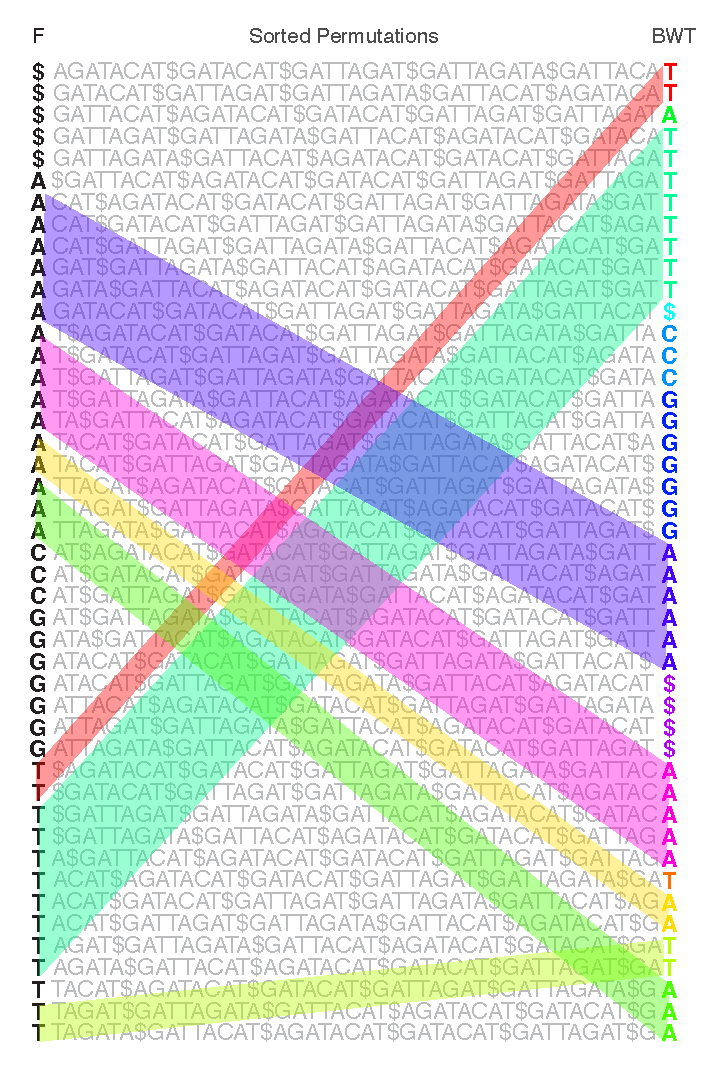
\includegraphics[width=0.5\linewidth]{Images/bwt_tag.pdf}
    \caption[An illustration of the Burrows Wheeler matrix]{An illustration of the Burrows Wheeler matrix (BWM) of the text T= GATTACAT\$AGATACAT\$GATACAT\$GATTAGAT\$GATTAGATA\$. BWM consists of T’s sorted rotations. The leftmost column is called F and the rightmost column is BWT(T), also called L. Distinct BWT runs are given distinct colors. The LF-mapping maps these runs to the same letter stretches in F. Colored parallelograms illustrate the LF mapping for runs of characters A, and T.}
    \label{fig:2:1}
\end{figure}

\subsection{Tag Arrays}
Rossi et al. \cite{rossi2022moni} recently introduced a pangenomic index for finding maximal exact matches (MEMs). This index allows finding MEMs of a given pattern P[1..m] in O(mlogn) time and listing the occurrences of each MEM in constant time per occurrence. This method enables the compact indexing of pangenomes, eliminating the risk of false positives and allowing for quick identification of good seeds and efficient listing of their occurrences.\\
However, a practical issue with Rossi et al.'s method is that in a pangenome containing thousands of genomes, a MEM can occur thousands of times across these genomes, even if all occurrences map to a single location in a standard reference genome. This complexity makes extending the seeds and combining the approximate matches of the reads more difficult.\\
Bal´az et al. \cite{balavz2024wheeler} showed how we could combine Rossi et al.'s method with a pangenome graph using tag arrays. They showed that this method still has Rossi et al.'s features in finding the seed quickly with no chance of false positives. But then, using the tag arrays, we are able to report the reads of non-chimeric occurrences in the graph in constant time per occurrence. \\
In the Wheeler map model, each text suffix T[i..] is labeled with a "tag", which can also be seen as labeling the positions of T. The tags of T are collected in a "tag array." In the Wheeler map, tags are the identifier of the nodes. Either the node or the edge that the T[i..] is correspond to. For example, In Figure \ref{fig:2:2}, the range for P = 'T' on the BWM is from index 33 to 45, and Tag[33..45] contains the tags 8, 4, and 3 which are the nodes that the T[i..] departs from. These tags are the labels that P appears in the graph. 
\begin{figure}
    \centering
    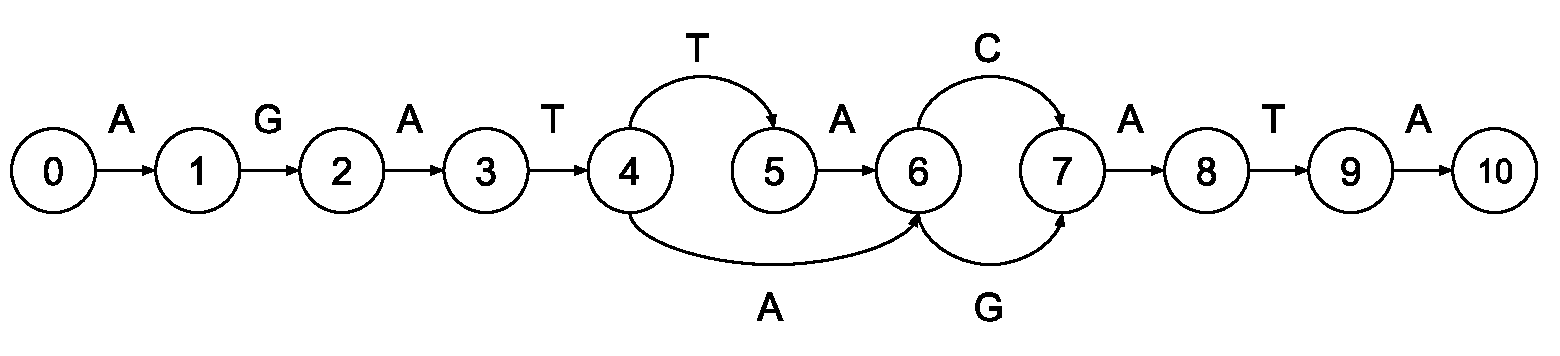
\includegraphics[width=\linewidth]{Images/Basic graph.pdf}
    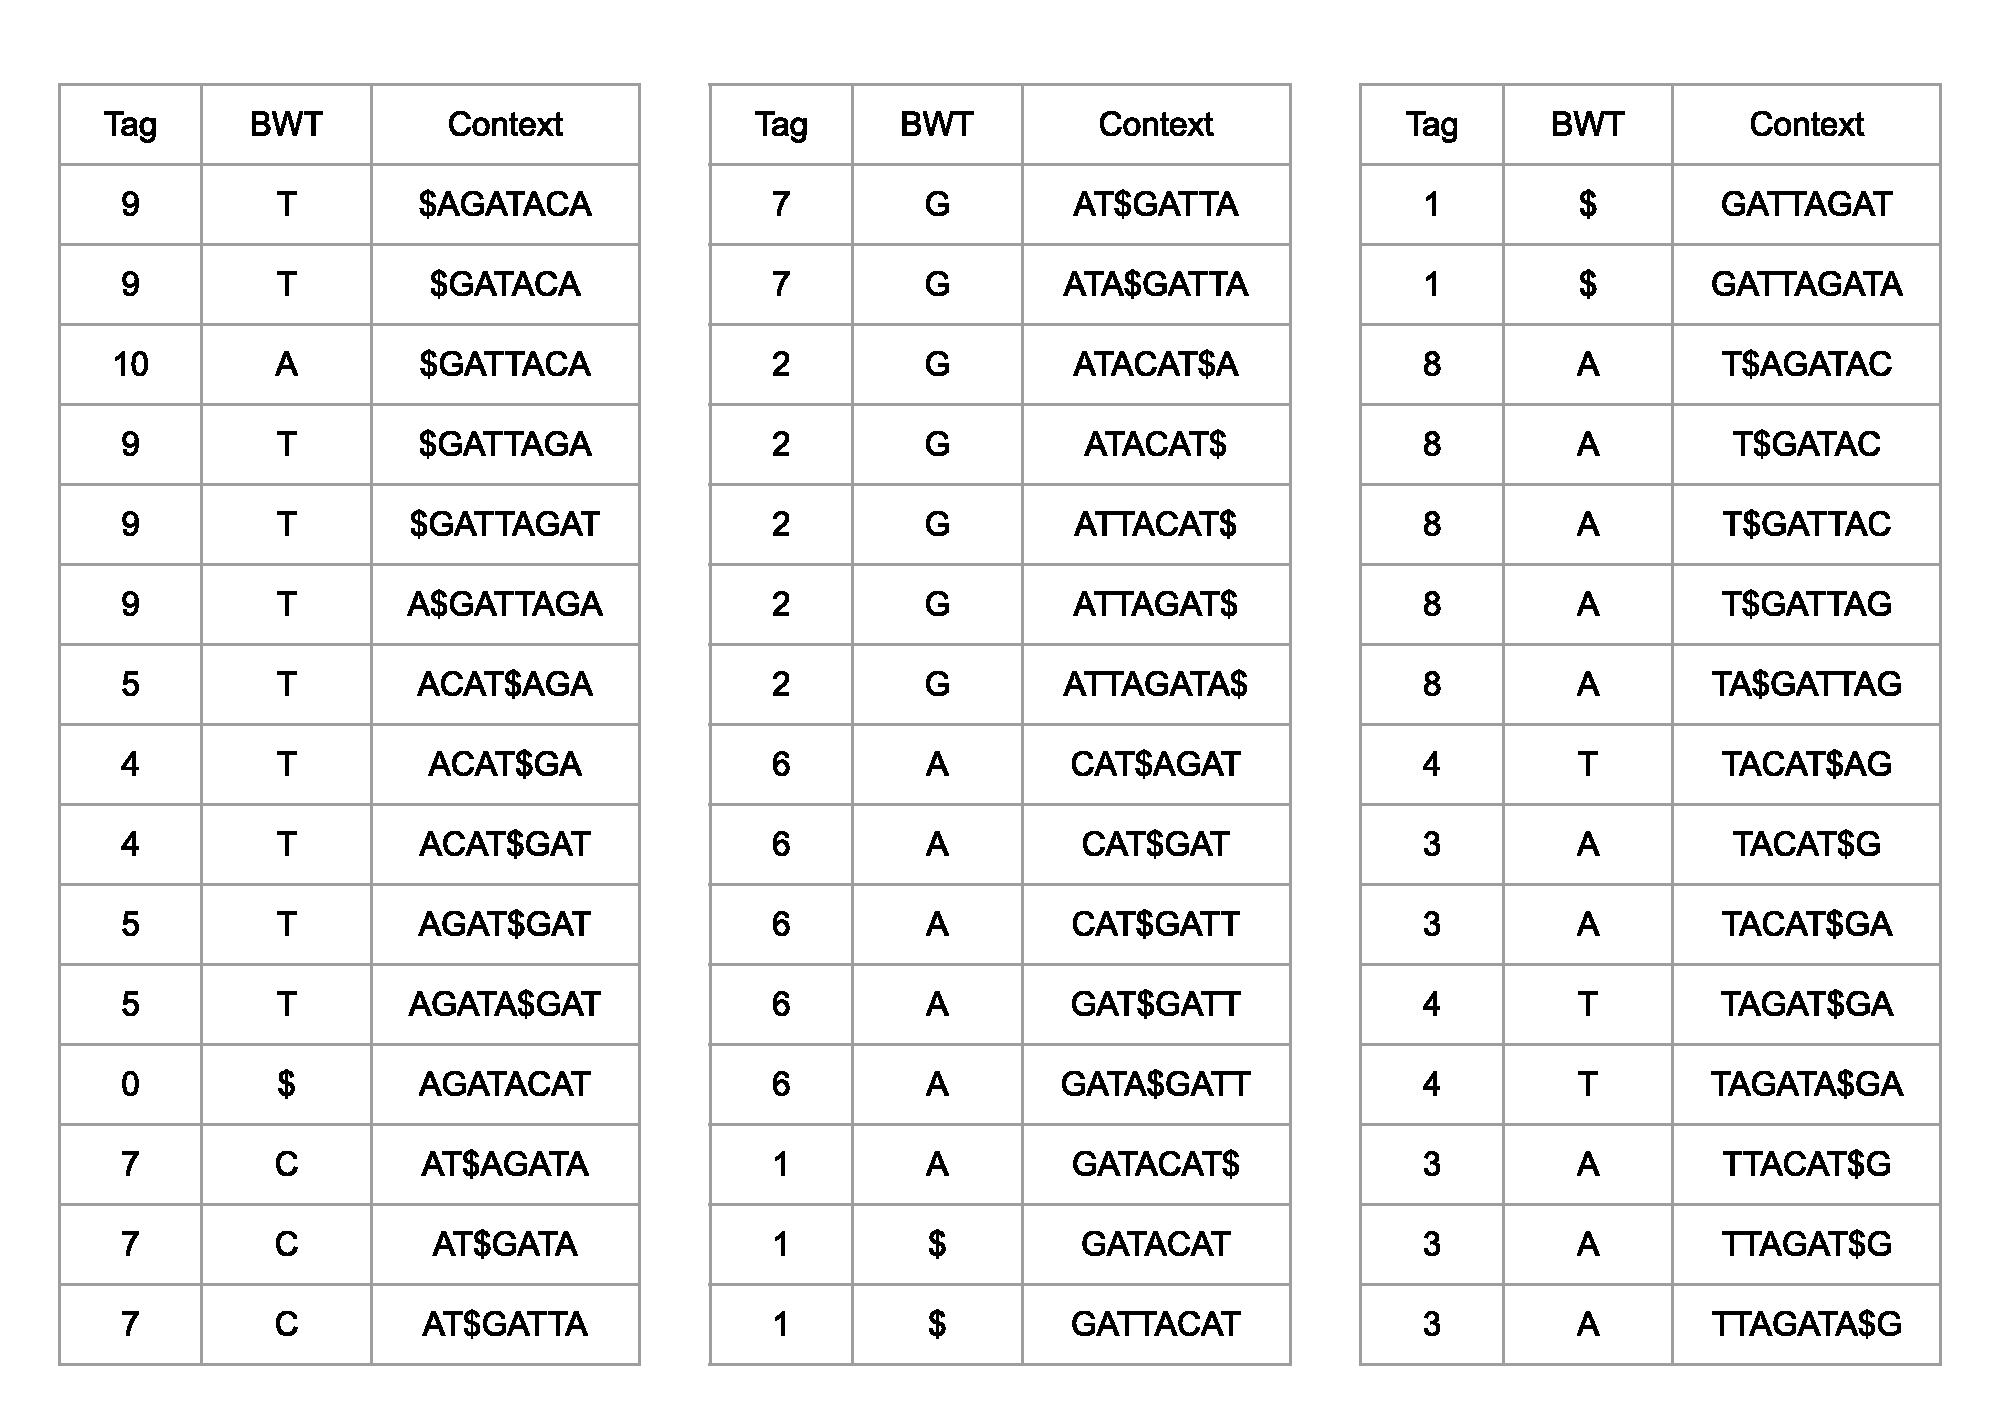
\includegraphics[width=\linewidth]{Images/Tag Arrays.pdf}
    \caption[Tag arrays for a simple graph]{This figure shows a toy genome graph on the top. The bottom tables shows the tag arrays for T = GATTACAT\$AGATACAT\$GATACAT\$GATTAGAT\$GATTAGATA\$. The tags in the first columns of the tables are the nodes that the correspond BWT character departs from. The right columns shows the text context which is the first few characters after the BWT characters.}
    \label{fig:2:2}
\end{figure}

\subsubsection{Tag arrays in pangenome graph}
The text we used as T in Figure \ref{fig:2:2} as an example, is the concatenation of different paths of the graph with separator "\$". We can build this text T in pangenomes by extracting the haplotype sequence information from the graph and concatenating them with "\$" between each two. Also, the other difference between the toy graph shown in Figure \ref{fig:2:2} and the pangenome variation graph is that the nodes contain the sequences (not the edges). We change the tags from numbers to positions on the graph, which can be defined as tuples (Node\_id, Offset, is\_rev) as used in vg. Each position on the variation graph can be addressed using node\_id (a unique identifier of the node), offset (a number addressing the specific base in the node), and is\_rev (which shows the direction that we are working with). From now we show the graph positions with variable $g$. The Figure \ref{fig:2:3} shows how a pangenome graph is represented. The red arrows map the nodes from the toy graph to the comparable positions on the toy pangenome graph. 

\begin{figure}[h]
    \centering
    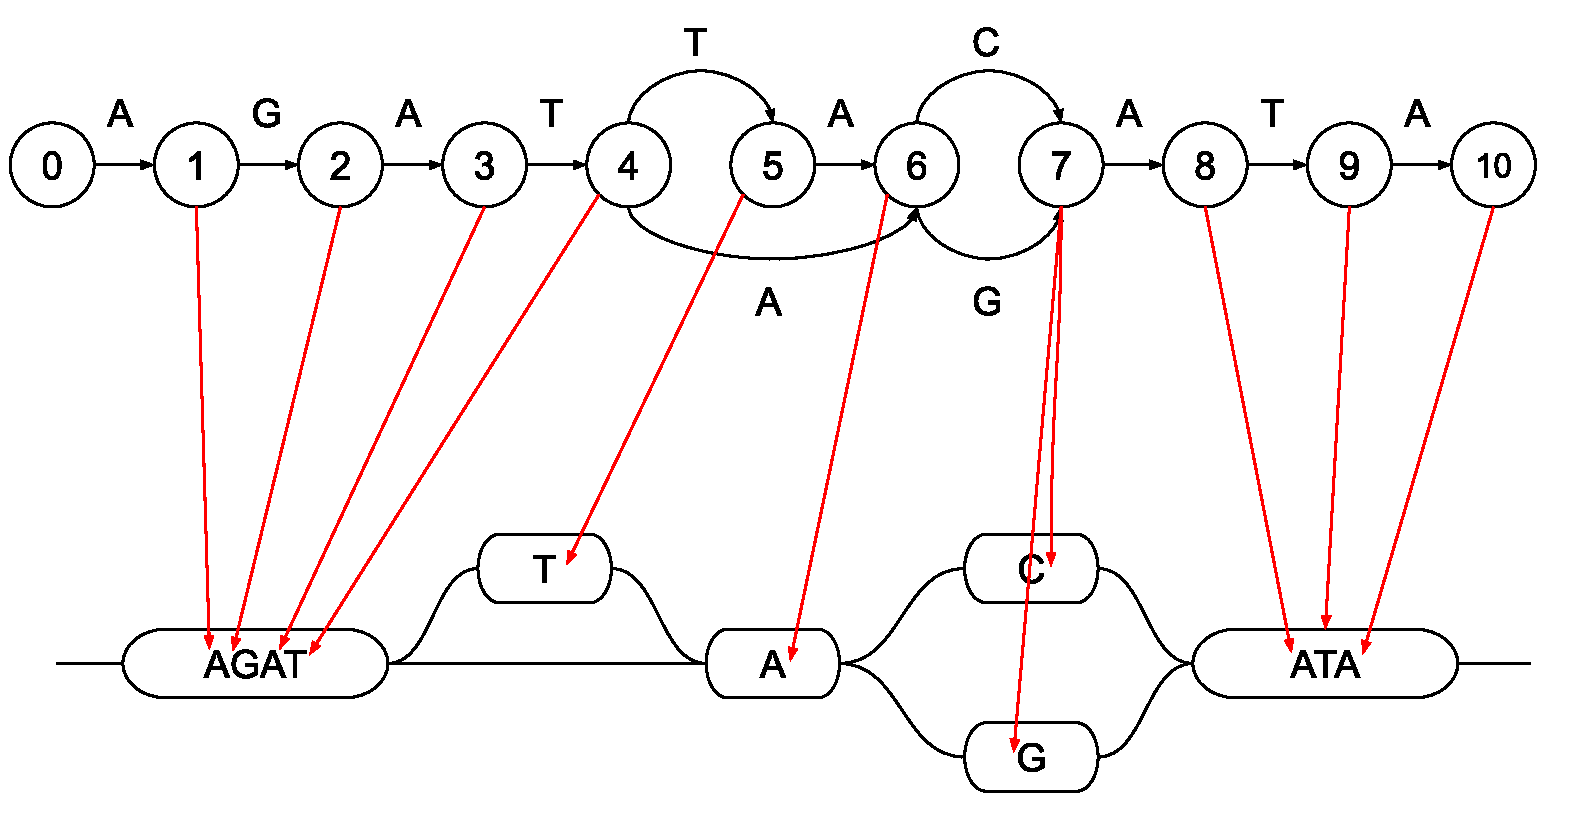
\includegraphics[width=\linewidth]{Images/Pangenome Graph.pdf}
    \caption[Mapping simple graphs to pangenome-like graphs]{Top graph is the same toy graph used in the previous figure. Bottom graph shows the equivalent pangenome-like illustration of the same graph.
}
    \label{fig:2:3}
\end{figure}

\subsection{B+ Tree}
A B+ tree \cite{comer1979ubiquitous, knuth1997art} is a self-balancing tree data structure that maintains sorted data and allows for efficient insertion, deletion, and search operations. As a type of balanced tree, a B+ tree ensures that the tree remains balanced, meaning all leaf nodes are at the same level. Therefore, it guarantees predictable and optimal performance for operations. This balancing property is achieved through the splitting and merging of nodes during insertions and deletions. This ensures that the tree height grows logarithmically with the number of elements, which keeps search operations efficient.\\
In a B+ tree, all values are stored at the leaf level, with internal nodes containing only keys that act as guides for navigating the tree. This structure makes B+ trees particularly efficient for range queries and sequential access, as the leaf nodes are linked together in a linked list, allowing for quick traversal of contiguous data. B+ tree remains balanced by splitting or merging nodes whenever the number of node items reaches a threshold. \\
B+ trees have a high fan-out (the number of children per node), which reduces the tree height. Therefore, it minimizes the number of disk accesses required during operations. This property make them ideal for database and file system indexing, where efficient data retrieval is crucial. The high fan-out and balanced nature of B+ trees ensure that operations such as search, insertion, and deletion are performed in O(log⁡n) time, where n is the number of elements in the tree. This efficiency, combined with their ability to handle large volumes of data and perform range queries efficiently, makes B+ trees a good choice for applications requiring fast and reliable access to sorted data.\\
As shown in Figure \ref{fig:2:4}, each non-leaf node i in the B+ tree that contains $N_i$ items, has $N_{i} + 1$ children (pointers to other nodes), and each leaf node j that has $N_j$ items, also has $N_{j} + 1$ pointers with the difference that the last pointer goes to the next node and other $N_j$ pointers hold the values of items. 

\begin{figure}[h]
    \centering
    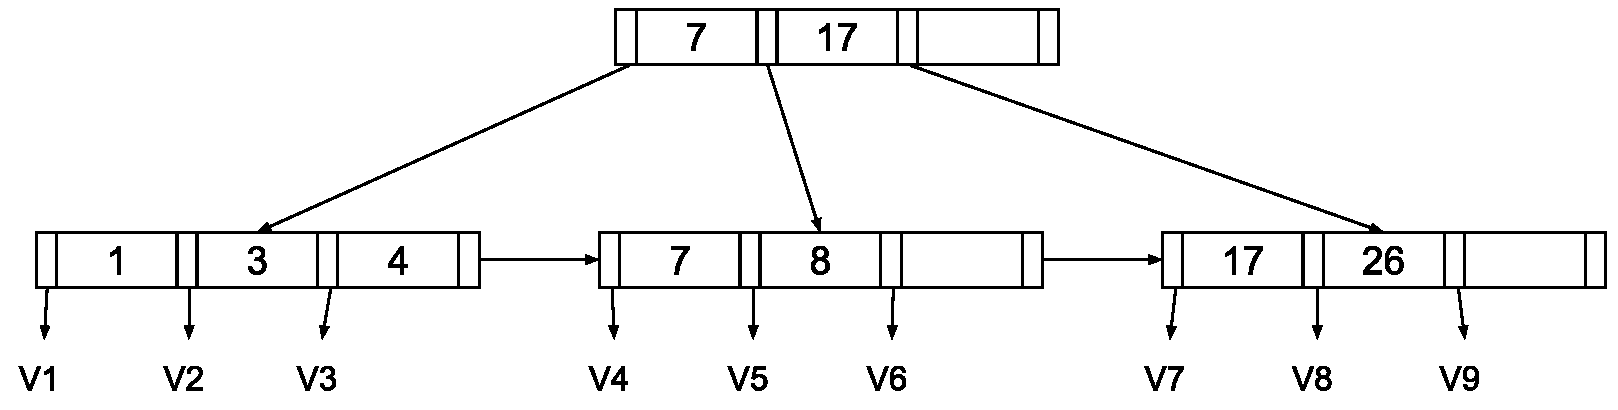
\includegraphics[width=\linewidth]{Images/B+ Tree Normal.pdf}
    \caption[B+ tree illustration]{An example of a B+ tree. This B+ tree contains 7 keys in the leaves that point to 9 values. }
    \label{fig:2:4}
\end{figure}

\section{Methods}

\subsection{Naive algorithm}

Building tag arrays is a demanding task, requiring a lot of memory and CPU time. The naive algorithm of building the tag array starts with the inverse suffix array (ISA). An ISA is the inverse mapping of the suffix array. In other words, if the suffix of T starting at position i (T[i..]) corresponds to the k-th index of the BWM, then $ISA[i]=k$. By traversing all the haplotypes in the pangenome graph and producing the ($ISA[i]$, $g_i$) for each text position T[i] and then sorting all these pairs by the first component we get (i, TAG[i]). This naive algorithm requires an extensive amount of memories (1000GiBs for with current pangenomes).  

\subsection{Run-Length B+ tree (RLBPT)}
One way to keep the tag arrays in an efficient space, is to run-length compress them. To maintain these run-length tag arrays, we need a data structure. This data structure can store and handle the run-length encoding while having efficient insertion, search, and deletion. \\
I designed and implemented a run-length b+ tree. This tree can efficiently search, delete, and insert run-length encoded tags in the tree. The basic concept of RLBPT and B+ tree is the same. Adding to the RLBPT requires extra steps. A Run is a pair of BWT index position and a graph position [index, $g_i$]. The Run also needs a length to be meaningful. A Run [I, $g_i$] with length $L_i$ means that from BWT position I to position $I + L_i$, all the graph positions are $g_i$.\\ 
Figure \ref{fig:2:5} shows a simple example of a RLBPT. RLBPT don't store the length of the Run as an extra variable. We added another special Run that we call Gap. A Gap is a Run but with graph position 0 (a special value that does not happen in the graph). The Gap Run is used to determine the end of the Run. So when adding a Run [I, $g_i$]  with length $L_i$, we also add a Gap [$I + L_i$, \mathcal{0}] so that we can calculate the length of the actual Run without needing an extra variable. \\
The main internal difference between this RLBPT and the B+ tree is in the insert function. The insert function of the RLBPT takes a Run and a length to add to the tree. Then it add a main run and a gap run to the tree. The whole concept of insert function is the same in both RLBPT and B+ tree. But, the difference is that in the RLBPT, the Runs can reach each other and merge if they have the same graph positions.
Because of the possibility of merging between runs, the nodes can underflow in the RLBPT. So, there is an extra step compared to the B+ tree. The underflow functionality is the same as underflow that happens in deletion in B+ tree. 
\begin{figure}[h]
    \centering
    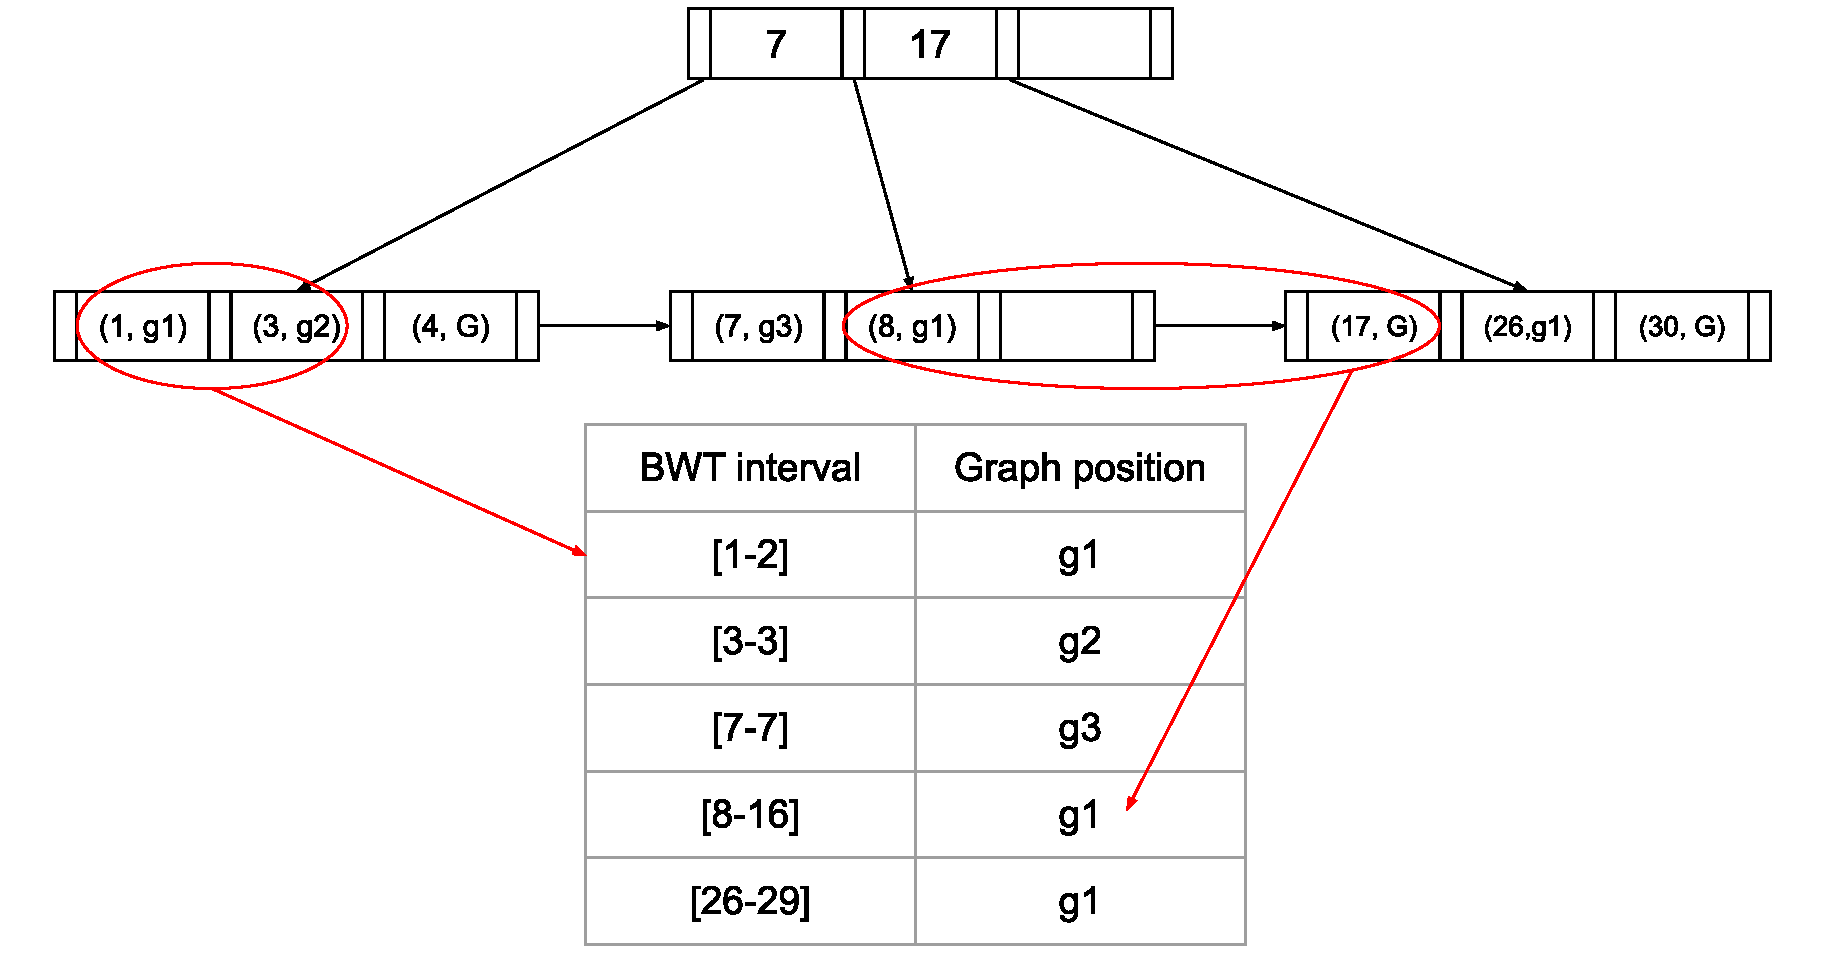
\includegraphics[width=\linewidth]{Images/RLBPT.pdf}
    \caption[Run-length B+ tree]{The top figure is a simple RLBPT and the table below shows the extracted BWT interval graph positions from the tree. The red arrows illustrate how the BWT intervals and graph positions can be queried from the tree. }
    \label{fig:2:5}
\end{figure}

\subsection{Unique K-mer indexing}
We call the k-mers that occur once in the graph, unique k-mers. We calculate these unique k-mers exactly like how Siren et al. \cite{siren2023personalized} calculate them (Aim1).
\subsubsection{Tags from unique k-mers}
I build an index for the pangenome unique k-mers. Now, for each k-mer X in the index with graph position $g_i$, the tag array interval corresponding to the BWT interval for X is a run of $g_i$. So, we can add the tags calculated from each unique k-mer to the RLBPT. We expect this algorithm of calculating the k-mers to be so much faster than the naive algorithm. \\
Figure \ref{fig:2:6} left table illustrates this algorithm and shows which positions of the tag arrays are covered by unique 4-mers. This strategy for this simple example covers 15 tags out of 45 tags possible.
\subsubsection{Extending the unique k-mers}
Another step in the algorithm is to extend the current unique k-mers by their predecessor character on the graph. Suppose X is a unique k-mer on the graph, and the only predecessor of that k-mer on the graph is a character y. In that case, the yX is also a unique k-mer on the graph. We can calculate the BWT interval of yX by finding the interval of X on the BWT (by searching the RLBPT) and find the yX interval using LF mapping. Then insert that interval into the RLBPT again. This method helps cover more tag arrays without needing to calculate them naively. \\
Figure \ref{fig:2:6} right table illustrates a simple example of extending k-mers. By extending the 4-mers with only one character, five more tags are getting covered. \\
I continue extending the unique k-mers using a BFS-like algorithm. First, I put all the intervals in a queue. Then, I try to extend k-mers with each of \{'A', 'T', 'C', 'G'\} and continue adding the ones that give us more unique positions into the queue until the queue is empty. 

\begin{figure}[h]
    \centering
    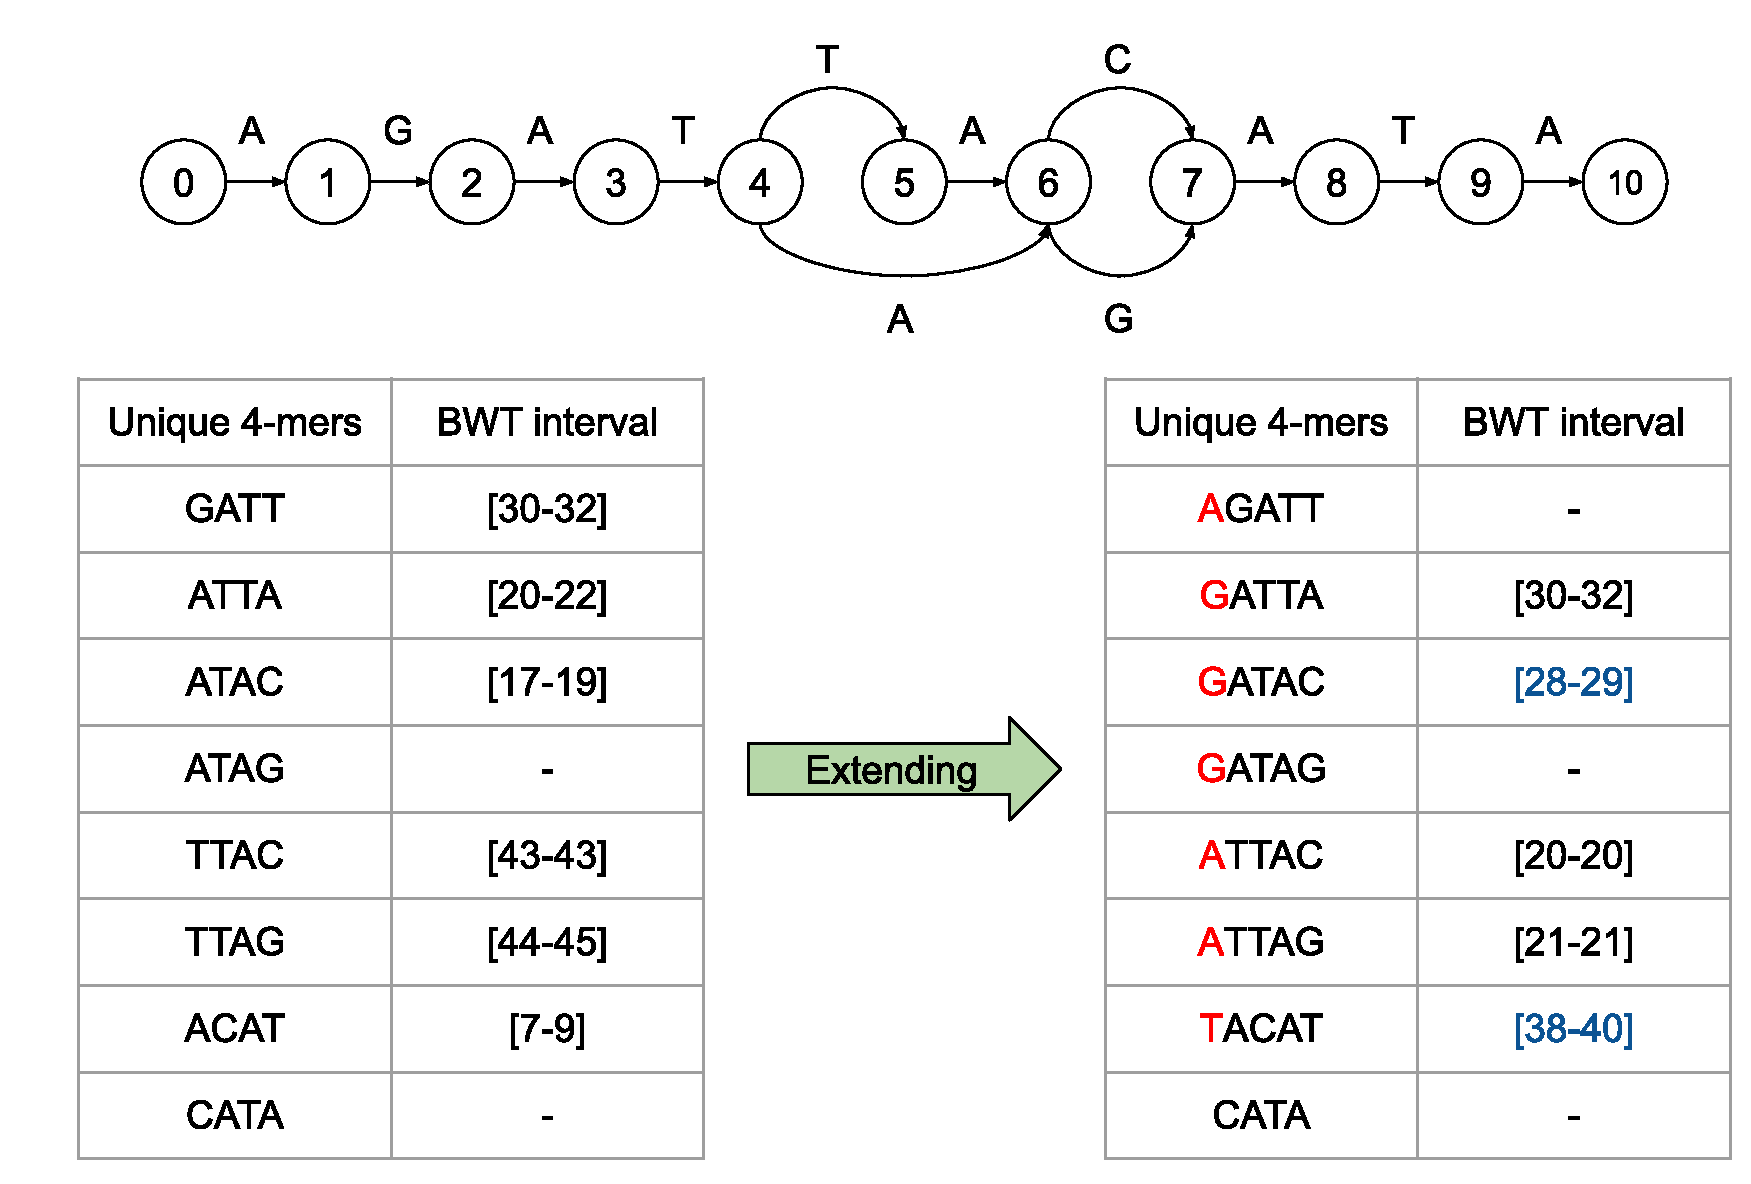
\includegraphics[width=\linewidth]{Images/Unique kmers.pdf}
    \caption[Unique k-mers algorithm example]{This is an illustration of using unique k-mers to find the tag arrays with the simple graph on top and T = GATTACAT\$AGATACAT\$GATACAT\$GATTAGAT\$GATTAGATA\$.The left table shows all the unique 4-mers of the simple graph and their BWT intervals. The right table is the result of extending the unique 4-mers by one character wherever possible. 
}
    \label{fig:2:6}
\end{figure}

\subsection{Filling the gaps}
After all these steps, there might still be positions on the haplotypes not covered by this method. We fill these parts using the naive algorithm. 

\subsection{Indexing and Merging Chromosomes}
To efficiently build the whole-genome index, we will first create per-chromosome tag arrays before merging them into a comprehensive whole-genome tag array. Smaller arrays are less resource-intensive, allowing us to manage memory usage more effectively. Additionally, the proposed kmer-based methods perform better with smaller arrays, as they can fill a larger fraction of the arrays, leading to faster and less memory intensive indexing. \\
The process of merging the per-chromosome tag arrays involves leveraging a whole-genome r-index. The r-index facilitates iteration over the suffix array, providing suffix array (SA) values at each position that can be converted to chromosome identifiers. This conversion helps determine the interleaving order of the per-chromosome tag arrays, effectively guiding the merging process. By using the r-index to map the interleaving of individual tag arrays, we can construct a cohesive whole-genome tag array. It is essential to ensure that the relative order of sequences remains consistent between the per-chromosome BWTs and the whole-genome BWT to maintain accuracy. \\
Merging and interleaving the tag arrays require a multi-string BWT approach. We will use grlBWT \cite{diaz2023efficient}, a linear-time semi-external algorithm for building the BWT of a string collection.



\section{Preliminary results}
I have tested the memory usage and efficacy of the unique k-mer and extending methods. I used specific graphs for each chromosome and found the unique k-mers. Then, for each unique k-mer, I used the RLBWT to find the BWT intervals corresponding to the k-mer sequence. Then, I added them to the RLBPT and checked the coverage of the tag arrays. \\
Figure \ref{fig:2:7} left plot shows the tag array coverage of the unique k-mer indexing before and after extending. The average tag array coverage after both steps is about 88\%, which shows the potential of this method in calculating the tag arrays. \\
Another critical measure is the memory usage of the algorithm. Figure \ref{fig:2:7} right plot shows the memory usage for each chromosome. The naive algorithm's memory usage is more than four times the memory usage of the proposed algorithm. 


\begin{figure}
    \centering
    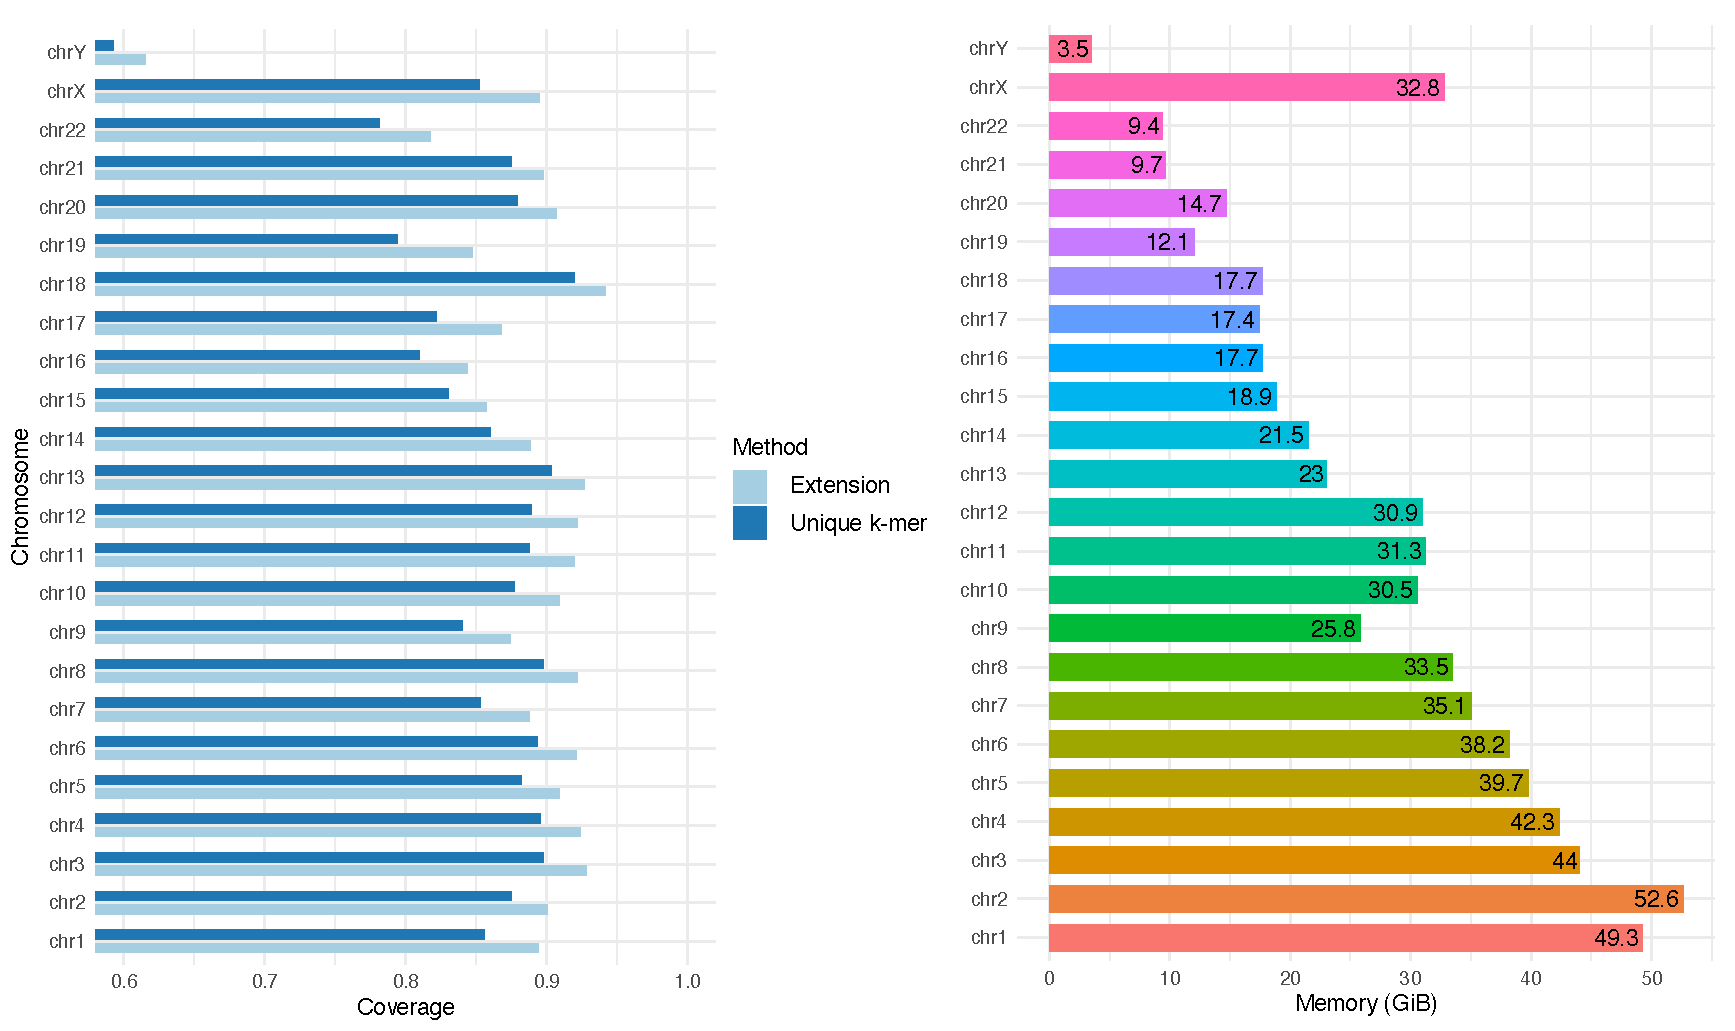
\includegraphics[width=\linewidth]{Images/results.pdf}
    \caption[Tag array coverage and memory usage]{Left plot shows the coverage of the proposed algorithms for building tag arrays. The right plot is the memory usage of algorithm including all steps of the algorithm. }
    \label{fig:2:7}
\end{figure}

\section{Expected outcome and evaluation}
The proposed graph indexing method using haplotype information is expected to revolutionize the efficiency of genomic data retrieval and analysis within pangenomes. One crucial analysis is that this method enhances the read sequence mapping to the pangenome. With multiple innovative algorithms, this method aims to significantly reduce the memory footprint traditionally required for indexing pangenomic data. We expect to be able to index high haplotype-numbered pangenomes using much less memory and CPU than the current methods. \\ 
I will use both the current HPRC pangenome release, which has 47 human genomes, and the next release from later 2024, which will have 150 human genomes embedded. I will measure this algorithm's CPU and memory usage and compare it with the current methods. Also, checking if the algorithm scales to bigger pangenomes is necessary, so I will use different versions of the HPRC pangenomes and check if the index grows so that we can use it with thousands of genomes.
As it is important for this graph indexing method to be universal, it has to work with data from different sources. So, I will also test the performance of this method using 1000 Genome Project \cite{10002015global} data by building the graph using vg and testing the indexing method with that. \\
I will compare the accuracy, memory efficiency, and the query processing time of the tag array indexing with other existing pangenome graph indexing methods from vg such as GCSA \cite{siren2017indexing}, GBWT index \cite{siren2020haplotype}, and minimizer indexing \cite{siren2021pangenomics}. We expect the tag array indexing to have superior performance. \\
I will evaluate the accuracy of this tool in locating and retrieving specific genomes. This evaluation will involve comparing the results of genomic queries against a known reference to ensure that the indexing method provides precise and reliable outcomes. I will create simulated queries from known parts of the DNA and calculate the accuracy of the indexer based on the truth positions.

\section{Project timeline}
I have already implemented tag array listing tools as a contribution to vg. I tested the unique k-mer algorithm on separate chromosomes to ensure this method would work. We are still designing the algorithm to merge the tag arrays from different chromosomes. I plan to finish the merging step before Fall 2024. Then, I plan to make a stand-alone tool that can be used without having the burden of compiling a big project such as vg. This will help any researcher to use the tag array indexing method. I plan to finish a complete graph indexing tool before the summer of 2025. 

 

\chapter{Aim3: Improving Moni-align with tag arrays}

\section{Introduction}
Current pangenome graph mappers, such as vg map \cite{siren2020haplotype} and vg Giraffe \cite{siren2021pangenomics}, have significantly improved read alignment accuracy by leveraging the rich information contained within pangenomes. These mappers utilize variation graphs and support various types of genomic data. However, graphs can quickly become complex as the size of pangenome grows. With the pangenome graphs, it is possible to create chimeric sequences in the graph that consist of known alleles but are not observed in nature. This will result in alignments to haplotypes that do not actually exist in the pangenome. \\
Moni-align \cite{rossi2022moni} introduces an r-index-based approach to pangenome alignment, utilizing a seed-and-extend strategy with Maximal exact matches as seeds. Maximal exact matches (MEMs) \cite{rossi2022moni}, which are exact matches between a read R and genome G that cannot be extended to the left or right, have been shown to be the most effective seeds for alignment of both short reads \cite{li2013aligning} and long reads \cite{vyverman2015long,miclotte2016jabba}.\\
While Moni-align demonstrates accuracy on par with leading aligners like VG and Giraffe, it faces issues with high memory requirements and slower alignment speeds when aiming to find exhaustive MEMs. To manage this, Moni-align employs filtering strategies, such as capping the number of MEM occurrences per genome and applying frequency-based filtering, sometimes resulting in the loss of informative reads (Moni-align has not published yet, and I will cite the authors' theoretical MONI paper and further information were through personal communication with the authors).\\
In this aim, I will contribute to Moni-align. I propose developing a novel MEM-finding mapping algorithm that leverages tag arrays to address these limitations. By using tag arrays for efficient and distinct MEM identification, our approach aims to enhance the accuracy and speed of read alignment while reducing memory usage. This method focuses on maintaining the informative reads by utilizing the structural advantages of tag arrays, thus optimizing the overall alignment process.

\section{Background}
Moni-align is a pangenome read aligner that utilizes the r-index, a novel approach for handling genomic alignments. It employs a seed-and-extend strategy, where MEMs are used as seeds for aligning reads to the pangenome. This method benefits from recent advancements that enhance the efficiency of MEM finding by augmenting the r-index with a small auxiliary threshold data structure. Moni-align aligns reads to the pangenome and then maps these alignments back to a linear reference genome, ensuring that the resulting SAM files are compatible with existing downstream analysis software.\\
Moni-align constructs the r-index from a FASTA file(s) and a VCF file using Prefix-free Parsing method. Although Gagie et al. \cite{gagie2020fully} showed that the r-index requires O(r)-space to be stored, they did not show how to efficiently build the r-index. This problem was later resolved via the introduction of a preprocessing technique called Prefix-free Parsing (PFP), which creates both a parse and a dictionary of the input which is then used to construct the r-index \cite{doi:10.1089/cmb.2019.0309,boucher2019prefix}\\
While the r-index performs exact pattern matching efficiently, it innately lacks an efficient method for partial matching. This makes it necessary to find MEMs. Moni-align uses a Threshold data structure to guide the r-index to continue a partial match when the backward search range becomes empty (when there is no perfect match) \cite{bannai2020refining}.\\
In the alignment step, Moni-align finds the MEMs between the read and the genome(s). It calculates all MEMs of any length using a simple two-pass algorithm that calculates matching statistics. Calculating all MEMs is ideal for the best alignment, but this approach quickly becomes impractical due to high memory requirements and significant alignment slowdowns \cite{roberts2004reducing}. \\
Currently, Moni-align is using various filtering approaches to reduce the MEM space. Moni-align retains a constant number of occurrences of a particular MEM per genome. Then, it also prunes the uninformative MEMs based on the frequency filter to reduce the MEM space even more. Applying the correct filter is hard, and ensuring no informative MEM is left out with a frequency filter method is impossible. 

\section{Method}
I will integrate the tag array indexing into Moni-align by creating a tag array index from the inputs of Moni-align and, later, calculating the MEMs and filtering them; I will use the tag array index to retain only the informative MEMs. This will help reduce the memory usage of Moni-align while pruning only the uninformative MEMs. \\
\subsection{Index construction}
Creating the tag array index requires a variation graph and the r-index. The r-index is already getting created in the Moni-align. I will create the variation graph required for the tag array index using vg construct \cite{garrison2018variation} or the user input. Then I will build the tag array index. (Figure \ref{fig:3:1}) This index can be used in the alignment step, to filter the MEMs. The tag array index cannot run with the r-index simultaneously, as the r-index is one of the inputs required for building the tag arrays. So this will add to the CPU time Moni-align needs to build the index. However, this is done only once and during the preprocessing step. 
\begin{figure}[h]
    \centering
    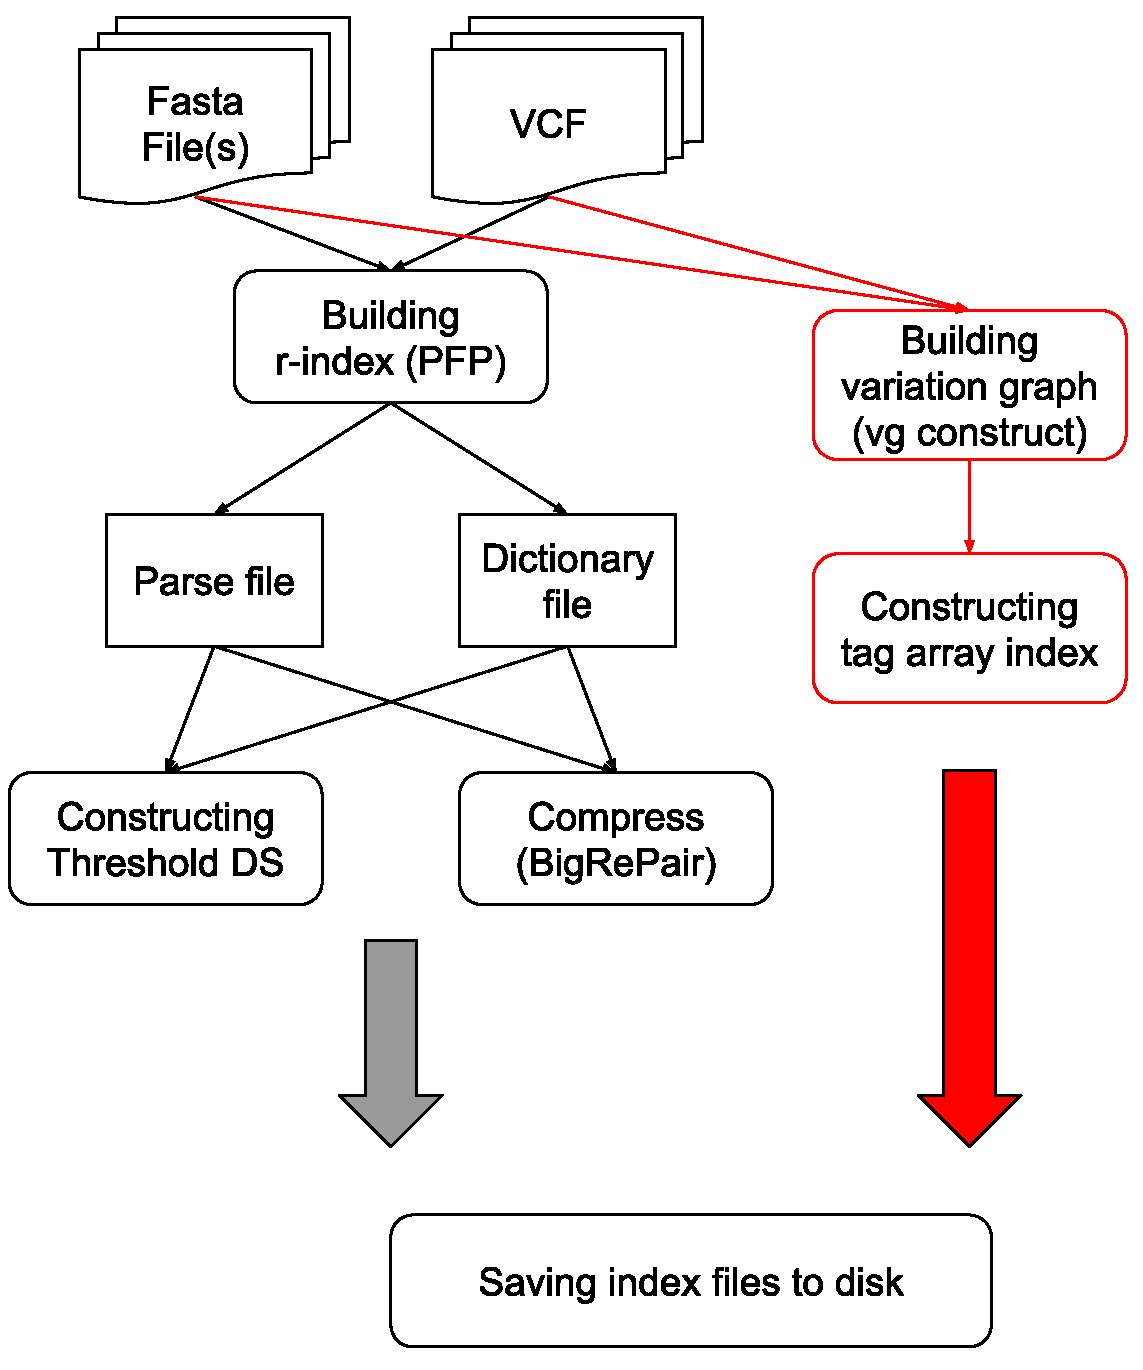
\includegraphics[width=0.6\linewidth]{Images/moni-build.pdf}
    \caption[Index construction in Moni-align with tag arrays]{Overview of the index construction in Moni. The black boxes and arrows illustrate the current index building proccess in Moni-build. The red boxes and arrows shows how the tag array index gets integrated into this approach.}
    \label{fig:3:1}
\end{figure}
\subsection{MEM filtering}
Instead of filtering based on frequency, we will use the tag array index to list a given pattern's distinct and informative MEMs. This filtering helps us keep all the informative MEMs while pruning all the uninformative ones. Keeping just the informative MEMs reduces the memory usage of the algorithm. Also, it helps improve the accuracy of the mapping, as it does not blindly remove a part of the informative reads. 

\section{Expected outcome and evaluation}
We expect this method to reduce the memory usage of Moni-align and also increase the mapping accuracy. Also, with this method, Moni-align will be able to use far bigger pangenomes. This could help reduce the biases in read mapping even more and reach the high accuracy needed for human genome analysis. \\
I will compare the performance of the proposed algorithm with other pangenome aligners, such as vg map \cite{garrison2018variation}, vg giraffe \cite{siren2021pangenomics}, and GraphAligner \cite{rautiainen2020graphaligner}. I will also compare this method with standard aligners, including Bowtie2 \cite{langmead2009ultrafast}, BWA, and Minimap2 \cite{li2018minimap2}. I will simulate short-read paired-end reads from 1000 Genome Project and measure the accuracy, memory usage, and scalability of all the methods with these reads. We expect high-accuracy mapping results while spending less memory than other methods. 


\bibliographystyle{plain}
\bibliography{uctest}


\end{document}
